\section{Matrix Factorization}  \label{sec:mf}


% need update and to be consistent with related work 
The essence of Matrix Factorization~(MF) is to learn the latent factors from observed entries in the matrix, and use them to predict unobserved entries. MF is one of the most successful models in domains like Collaborative Filtering~(CF) in recommendation systems. In CF, the rows of the matrix are users and the columns are items, and we want to predict unknown rating scores that reflect users' preference to items. The unknown rating prediction in CF is equivalent to missing data recovery in Wireless Sensor Network~(WSN), except the rows become time frames, the columns become sensor nodes, and the data characteristic is different. 

In the following, we will first introduce the basics of MF. Then we will talk about how we modify the objective function of MF and make it adapted to the WSN data, and finally the complete procedure of our proposed method.

\subsection{Basic Formulation of Matrix Factorization}

The idea of MF is strongly related to Singular Value Decomposition~(SVD). SVD decomposes a completely observed matrix~$\mathbf{R}$ into one diagonal matrix~$\mathbf{D}$ and two unitary matrix~$\mathbf{U}$ and~$\mathbf{V}$ such that
\begin{equation*} \mathbf{R} = \mathbf{U}\mathbf{D}\mathbf{V}^T. \end{equation*}
While keeping the largest K singular values, $\mathbf{U}_K \mathbf{D}_K \mathbf{V}_K^T$ is the best K-rank approximation of $\mathbf{R}$ under Frobenius Norm. 

Yet, conventional SVD is undefined when the matrix~$\mathbf{R}$ is incomplete. Recent research shows\cite{koren2009matrix} when the matrix~$\mathbf{R}$ is partially observed, a better approach is to factorize $\mathbf{R}$ by considering observed entries only. By some numerical optimization procedures, we obtain two small matrices~$\mathbf{P}_{MK}$ and $\mathbf{Q}_{KN}$ that approximate observed entries in the matrix~$\mathbf{R}_{MN}$
\begin{equation*}\mathbf{R} \approx \mathbf{P} \mathbf{Q}.\end{equation*}
If $\mathbf{R}$ is a matrix of temperature readings, then each row of $\mathbf{P}$ represents latent factors of the time frame and each column of $\mathbf{Q}$ is the latent factors of the sensor node.

Here we adopted the biased MF: row bias $\mu_m$ and column bias $\mu_n$ is added for predicting $r_{m,n}$. In a temperature monitoring system, the row bias can be understood as the average temperature at the time, and the column bias reflects the systematic bias of the sensor node. Therefore, our prediction $\hat{r}_{m,n} = \mu_m + \mu_n + \mathbf{p}_m \mathbf{q}_n$. After adding the regularization term, the whole objective function becomes
\begin{equation*}\begin{aligned}
\frac{1}{2}\sum_{m,n}{(r_{m,n} - \hat{r}_{m,n})}^2 & + \frac{\beta_1}{2}\sum_m{\mu_m^2} + \frac{\beta_2}{2}\sum_n{\mu_n^2}\\
& + \frac{\beta_3}{2}\sum_m{||\mathbf{p}_m||^2} + \frac{\beta_4}{2}\sum_n{||\mathbf{q}_n||^2}.\\
\end{aligned}\end{equation*}
In the equation, $\mathbf{p}_m$ is the row factors of $\mathbf{P}$ (for time $m$), and $\mathbf{q}_n$ is the column factors of $\mathbf{Q}$ (for sensor node $n$) respectively. $\beta_1$, $\beta_2$, $\beta_3$, $\beta_4$ are parameters that control the strength of regularization.

\subsection{Temporal Regularized Matrix Factorization}

\begin{figure}[htbp]
	\centering
	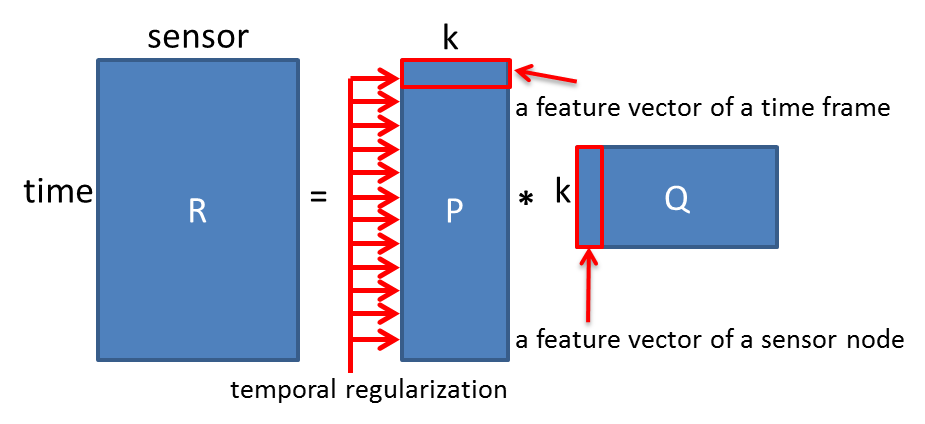
\includegraphics[width=0.5\textwidth]{TRMF_illustration.png}
	\caption{illustration of TRMF}
\end{figure}

%cite temporal reference

Although the goals of both CF and WSN data recovery are unobserved entry prediction, the data characteristics are very different. Firstly, in CF we have millions of users and items. In contrast, there are usually many time frames but few sensors in WSN. The spatial correlation of the sensors may be easily learnt from the data, but the temporal correlation is badly captured. Secondly, users and items are independent in CF, while time frames in WSN have a fixed order: closer time frames have stronger correlation. Having the observation, we come up with Temporal Regularized Matrix Factorization (TRMF) to better fit the characteristic of WSN data. 

TRMF adds a temporal regularization term on conventional MF. The temporal regularization forces the bias terms and features of adjacent rows to be similar, which reflects our intuition that readings in adjacent time frames should be similar. To be specific, we change our objective function into 
\begin{equation*}\begin{aligned}
\frac{1}{2}\sum_{m,n}{(r_{m,n} - \hat{r}_{m,n})}^2 &+ \frac{\beta_1}{2}\sum_m{\mu_m^2} + \frac{\beta_2}{2}\sum_n{\mu_n^2}\\
&+ \frac{\beta_3}{2}\sum_m{||\mathbf{p}_m||^2} + \frac{\beta_4}{2}\sum_n{||\mathbf{q}_n||^2}\\ 
&+ \frac{1}{2}\gamma_1\sum{(\mu_m-\mu_{m+1})^2} + \frac{1}{2}\gamma_2\sum{||\mathbf{p}_m-\mathbf{p}_{m+1}||^2}.
\end{aligned}\end{equation*}

\subsection{Optimization Procedure of TRMF}
\label{optimation_procedure}
Several approaches have been suggested for solving MF, like Stochastic Gradient Descent (SGD)\cite{koren2009matrix,chih2008large}, Alternating Least Square (ALS)\cite{koren2009matrix,zhou2008large} and Newton's method\cite{buchanan2005damped}. We adopt SGD for its efficiency and simplicity. 

In SGD, we incrementally update our model by considering one observed entry at a time. Focused on one observed reading $r_{m,n}$, the objective function of MF is
\begin{equation*} \frac{1}{2}(r_{m,n} - \hat{r}_{m,n})^2 + \frac{\beta_1}{2}\mu_m^2 + \frac{\beta_2}{2}\mu_n^2 + \frac{\beta_3}{2}||\mathbf{p}_m||^2 + \frac{\beta_4}{2}||\mathbf{q}_n||^2\end{equation*}
Thus, the update equation is\\
$\begin{cases}
	\mu_m' = \mu_m - \eta_1 ((\hat{r}_{m,n}-r_{m,n}) + \beta_1 \mu_m) \\
	\mu_n' = \mu_n - \eta_1 ((\hat{r}_{m,n}-r_{m,n}) + \beta_2 \mu_n) \\
	\mathbf{p}_{m}' = \mathbf{p}_{m} - \eta_2 ((\hat{r}_{m,n}-r_{m,n})\mathbf{q}_{n} + \beta_3 \mathbf{p}_{m})\\
	\mathbf{q}_{n}' = \mathbf{q}_{n} - \eta_2 ((\hat{r}_{m,n}-r_{m,n})\mathbf{p}_{m} + \beta_4 \mathbf{q}_{n})\\
\end{cases}$\\
After we use every rating in the training set once, we update the model according to the temporal regularization
$\begin{cases}
	\mu_u' = \mu_u - \eta_1 \gamma_1((\mu_u-\mu_{u-1})+(\mu_u-\mu_{u+1}))\\
	\mathbf{p}_{u}' = \mathbf{p}_{u} - \eta_2 \gamma_1((\mathbf{p}_{u}-\mathbf{p}_{u-1})+(\mathbf{p}_{u}-\mathbf{p}_{u+1}))\\
\end{cases}$

We summarize our algorithm in \textbf{Procedure \ref{alg:TRMF}}. Some details are explained in the following:

\paragraph*{Data Normalization}

Unlike the rating scores in CF are in a fixed range, readings from WSN are real-valued, and the range varies in different applications. Before training, we normalize the training set by its mean and variance, and in training we update the model by the normalized training set. While predicting validation set and testing set, we restore the prediction to the original mean and variance range and then calculate the error.

There are two benefits of data normalization. Firstly, when the global mean becomes zero, the origin of our model becomes a good initial point. The initial point impacts the performance of MF greatly because the objective function of MF is non-convex and we can only find the local minimum. Secondly, normalization makes different data sets look similar. It simplifies the parameter tuning task for TRMF and it is the foundation of Multivariate TRMF (Section \ref{subsec:Multivariate_TRMF}). 


\paragraph*{Initialization}

There are three ways to initialize the bias terms:
\begin{enumerate}
	\setlength {\itemsep}{-5pt}
	\item Set all of them to zeros.
	\item Set the row bias as the row mean, and then set the column bias as the column mean of every reading minus its row bias.
	\item The other way around.
\end{enumerate}
For all components of every $\mathbf{p}_{u}$ and $\mathbf{q}_{i}$, we set them as ~$\mbox{random}(-0.05,0.05)/K$, where $K$ is number of features.

\paragraph*{Parameters}

We seem to have many parameters: conventional regularization for user bias~$\beta_1$, item bias~$\beta_2$, user feature~$\beta_3$, item feature~$\beta_4$, temporal regularization term for bias~$\gamma_1$ and for feature~$\gamma_2$, learning rate for bias~$\eta_1$ and for feature~$\eta_2$, number of features~$K$, but in many cases we can achieve reasonable performance by setting 
\begin{equation*}\beta_1 = \beta_2 = \beta_3 = \beta_4, \gamma_1 = \gamma_2, \eta_1 = \eta_2. \end{equation*}
This is also our setting in the experiment. We share our experience about setting parameters in \textbf{Section \ref{subsec:parameter}}.

\paragraph*{Stopping Criterion}

We need to know when to stop updating the model. We use validation set and stop training if validation error is increasing and the current iteration number minus the best iteration number is greater than a threshold.  The iteration threshold here we choose 500. 

\begin{algorithm}
	\caption{Temporal Regularized Matrix Factorization}
	\label{alg:TRMF}
	\textbf{Parameter:} $\beta_1$, $\beta_2$, $\beta_3$, $\beta_4$, $\gamma_1$, $\gamma_2$, $\eta_1$, $\eta_2$, $K$\\
	\textbf{Input:} training set, validation set
	\begin{algorithmic}
		\State Normalize the training set as $\mathcal{D}$
		\State Initialize the $\mu_m$, $\mu_n$, $\mathbf{p}_m$, $\mathbf{q}_n$ for all $m$, $n$
		\Repeat
			\State \textbf{for} each observed reading $r_{m,n}$ in $\mathcal{D}$
				\State \indent Update $\mu_m$, $\mu_n$, $\mathbf{p}_{m}$, $\mathbf{q}_{n}$
			\State Update $\mu_m$, $\mathbf{p}_m$ for every $m$ by temporal regularization
		\Until{stopping criterion is met}
		\State Output the model for testing set prediction
	\end{algorithmic}
\end{algorithm}


